\documentclass{beamer}
\usepackage[utf8]{inputenc}
\usepackage{listings}
\usepackage{xcolor}
\usepackage{tikz}

\usetheme{Madrid}
\usecolortheme{default}

\definecolor{codegreen}{rgb}{0,0.6,0}
\definecolor{codegray}{rgb}{0.5,0.5,0.5}
\definecolor{codepurple}{rgb}{0.58,0,0.82}
\definecolor{backcolour}{rgb}{0.95,0.95,0.92}
\definecolor{rustblue}{rgb}{0.0,0.4,0.8}
\definecolor{solidityorange}{rgb}{1.0,0.5,0.0}

% Rust language definition
\lstdefinelanguage{Rust}{
    keywords={fn, let, mut, struct, enum, impl, trait, pub, use, mod, if, else, match, loop, for, while, break, continue, return, true, false, Some, None, Ok, Err, String, Vec, Box, Option, Result, u8, u16, u32, u64, u128, i8, i16, i32, i64, i128, f32, f64, bool, char, str, Self, self},
    keywordstyle=\color{rustblue}\bfseries,
    ndkeywords={unwrap, expect, clone, into, from, Default, Debug, Display},
    ndkeywordstyle=\color{magenta}\bfseries,
    sensitive=true,
    comment=[l]{//},
    commentstyle=\color{codegreen}\itshape,
    string=[b]",
    stringstyle=\color{codepurple},
    morestring=[b]',
}

% Enhanced Solidity language definition
\lstdefinelanguage{Solidity}{
    keywords={pragma, contract, function, modifier, event, struct, enum, mapping, address, uint, uint8, uint16, uint32, uint64, uint128, uint256, int, int8, int16, int32, int64, int128, int256, bool, byte, bytes, bytes1, bytes4, bytes8, bytes16, bytes32, string, fixed, ufixed, if, else, for, while, do, break, continue, return, throw, emit, require, assert, revert, new, delete, this, super, selfdestruct, suicide, sha3, keccak256, sha256, ripemd160, ecrecover, addmod, mulmod, now, block, msg, tx, public, private, internal, external, pure, view, payable, constant, anonymous, indexed, memory, storage, calldata, library, using, import, is, override, virtual, abstract, interface, try, catch, assembly},
    keywordstyle=\color{solidityorange}\bfseries,
    ndkeywords={true, false, wei, gwei, ether, seconds, minutes, hours, days, weeks, years},
    ndkeywordstyle=\color{magenta}\bfseries,
    sensitive=true,
    comment=[l]{//},
    morecomment=[s]{/*}{*/},
    commentstyle=\color{codegreen}\itshape,
    string=[b]",
    stringstyle=\color{codepurple},
    morestring=[b]',
}

\lstdefinestyle{mystyle}{
    backgroundcolor=\color{backcolour},   
    commentstyle=\color{codegreen}\itshape,
    keywordstyle=\color{magenta}\bfseries,
    numberstyle=\tiny\color{codegray},
    stringstyle=\color{codepurple},
    basicstyle=\ttfamily\footnotesize,
    breakatwhitespace=false,         
    breaklines=true,                 
    captionpos=b,                    
    keepspaces=true,                 
    numbers=left,                    
    numbersep=5pt,                  
    showspaces=false,                
    showstringspaces=false,
    showtabs=false,                  
    tabsize=2,
    frame=single,
    rulecolor=\color{codegray},
    identifierstyle=\color{black},
}

\lstset{style=mystyle}

\title{Zero-Knowledge Bug Bounty Program}
\subtitle{A Proof of Concept}
\author{Antonio Viggiano}
\date{\today}

\begin{document}

\frame{\titlepage}

\begin{frame}
\frametitle{Problem}
\begin{itemize}
    \item \textbf{Trust Issues in Bug Bounty Programs}
        \begin{itemize}
            \item Whitehats must reveal exploit details before payment
            \item Protocols may not pay after learning the vulnerability
            \item High risk for security researchers
        \end{itemize}
    \item \textbf{Need for Privacy-Preserving Vulnerability Reporting}
        \begin{itemize}
            \item Prove knowledge of an exploit without revealing it
            \item Cryptographic guarantees for fair exchange
            \item Minimize trust requirements between parties
        \end{itemize}
\end{itemize}
\end{frame}

\begin{frame}
\frametitle{Solution Architecture}
\begin{center}
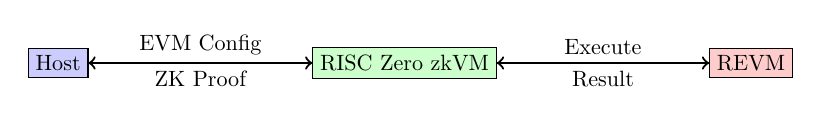
\begin{tikzpicture}[scale=0.8, transform shape]
    \node[rectangle, draw, fill=blue!20] (host) at (0, 0) {Host};
    \node[rectangle, draw, fill=green!20] (zkvm) at (5.5, 0) {RISC Zero zkVM};
    \node[rectangle, draw, fill=red!20] (revm) at (11, 0) {REVM};
    
    \draw[->, thick] (host) -- (zkvm) node[midway, above] {EVM Config};
    \draw[->, thick] (zkvm) -- (revm) node[midway, above] {Execute};
    \draw[->, thick] (revm) -- (zkvm) node[midway, below] {Result};
    \draw[->, thick] (zkvm) -- (host) node[midway, below] {ZK Proof};
\end{tikzpicture}
\end{center}

\begin{itemize}
    \item \textbf{Host}: Prepares bytecode and calldata, manages verification
    \item \textbf{zkVM}: Provides zero-knowledge execution environment
    \item \textbf{REVM}: Executes Ethereum Virtual Machine bytecode
    \item \textbf{Privacy}: Only hashes of inputs are revealed, not the exploit itself
\end{itemize}
\end{frame}

\begin{frame}[fragile]
\frametitle{Smart Contract Example}
\begin{lstlisting}[language=Solidity]
// Contract.sol
pragma solidity ^0.8.26;

contract Contract {
    function isSolved(int256 x) external pure returns (bool) {
        // p(x) = x^4 - 84x^3 + 1765x^2 - 84x + 1764
        return ((x**4)
            - (84 * (x**3))
            + (1765 * (x**2))
            - (84 * x)
            + 1764) == 0;
    }
}
\end{lstlisting}
\begin{itemize}
    \item Polynomial equation with specific roots
    \item Whitehat must find correct input value (x = 42)
    \item Function returns true for valid solutions
\end{itemize}
\end{frame}

\begin{frame}[fragile]
\frametitle{Host Implementation}
\begin{lstlisting}[language=Rust, basicstyle=\ttfamily\tiny]
fn main() {
    let config = EvmConfig::default();
    
    // Compute and display hashes for privacy
    let bytecode_hash = Keccak256::digest(config.get_bytecode());
    let calldata_hash = Keccak256::digest(config.get_calldata());
    
    println!("Executing bytecode hash: 0x{}", 
        hex::encode(bytecode_hash));
    
    // Execute inside zkVM
    let (receipt, return_value) = execute_evm_bytecode(config);
    
    // Verify the proof
    receipt.verify(REVM_GUEST_ID).expect("Verification failed");
    
    println!("Receipt verified! Result: {:02x?}", return_value);
}
\end{lstlisting}
\end{frame}

\begin{frame}[fragile]
\frametitle{Guest (zkVM) Implementation}
\begin{lstlisting}[language=Rust, basicstyle=\ttfamily\tiny]
fn main() {
    let config: EvmConfig = env::read();
    
    // Create EVM with in-memory database
    let ctx = Context::mainnet().with_db(CacheDB::<EmptyDB>::default());
    let mut evm = ctx.build_mainnet();
    
    // Deploy contract
    let deploy_result = evm.transact_commit(
        TxEnv::builder()
            .kind(TxKind::Create)
            .data(Bytes::from(config.bytecode.clone()))
            .build().unwrap()
    ).unwrap();
    
    // Call function with private calldata
    let call_result = evm.transact_commit(/* ... */);
    
    // Commit only hashes, not raw data
    env::commit(&(bytecode_hash, calldata_hash, is_solved));
}
\end{lstlisting}
\end{frame}

\begin{frame}
\frametitle{Privacy Features}
\begin{itemize}
    \item \textbf{Input Privacy}
        \begin{itemize}
            \item Bytecode and calldata are hashed using Keccak256
            \item Only hashes are committed to the proof journal
            \item Original exploit details remain secret
        \end{itemize}
    \item \textbf{Verifiable Execution}
        \begin{itemize}
            \item RISC Zero provides cryptographic proof of correct execution
            \item Anyone can verify the proof without trusting the prover
            \item Result integrity is mathematically guaranteed
        \end{itemize}
    \item \textbf{Zero-Knowledge Properties}
        \begin{itemize}
            \item Proves knowledge of a valid exploit
            \item Reveals nothing about the exploit method
            \item Enables trustless bug bounty programs
        \end{itemize}
\end{itemize}
\end{frame}

\begin{frame}
\frametitle{Current Implementation (Version 0)}
\begin{itemize}
    \item \textbf{Proof of Concept}
        \begin{itemize}
            \item REVM successfully runs inside RISC Zero zkVM
            \item Public bytecode with private calldata
            \item Commits code/calldata hashes and boolean outcome
        \end{itemize}
    \item \textbf{Key Components}
        \begin{itemize}
            \item Solidity compiler integration (build.rs)
            \item ABI encoding for function calls
            \item Hash-based privacy preservation
            \item Automated testing framework
        \end{itemize}
    \item \textbf{Verification Process}
        \begin{itemize}
            \item Host generates proof of EVM execution
            \item Proof can be verified by any third party
            \item Mathematical guarantee of correctness
        \end{itemize}
\end{itemize}
\end{frame}

\begin{frame}
\frametitle{Next Steps (Roadmap)}
\begin{itemize}
    \item \textbf{Version 1: Real Chain State}
        \begin{itemize}
            \item Anchor execution to real blockchain state
            \item Witnessed snapshot at specific block height
            \item Merkle Patricia Trie verification
            \item Fully explicit, deterministic TxEnv
        \end{itemize}
    \item \textbf{Version 2: On-Chain Integration}
        \begin{itemize}
            \item On-chain verification via RISC Zero verifier
            \item Predicate registry for vulnerability patterns
            \item Escrow vault for bounty payments
            \item Pay-to-reveal hash timelocked contracts
        \end{itemize}
\end{itemize}
\end{frame}

\begin{frame}
\frametitle{Questions?}
\begin{center}
\Large Thank you for your attention

\vspace{1cm}

\begin{itemize}
    \item Built as part of EF Core Program Brazil 2025
    \item Demonstrates ZK-EVM capabilities in RISC Zero
    \item Foundation for trustless bug bounty programs
\end{itemize}

\end{center}
\end{frame}

\end{document}
